% Adjust these for the path of the theme and its graphics, relative to this file
%\usepackage{beamerthemeFalmouthGamesAcademy}
\usepackage{../../beamerthemeFalmouthGamesAcademy}
\usepackage{multimedia}
\graphicspath{ {../../} }

% Default language for code listings
\lstset{language=C++,
        morekeywords={each,in,nullptr,int32, TCHAR, uint8, int8, uint16, int16,
        uint32, int32, uint64, int64, PTRINT, UObject. AActor, SWidget, FName,
        FString, UClass, USoundCue, UTexture}
}

% For strikethrough effect
\usepackage[normalem]{ulem}
\usepackage{wasysym}
\usepackage{listings}
\usepackage{pdfpages}

% http://www.texample.net/tikz/examples/state-machine/
\usetikzlibrary{arrows,automata}

\newcommand{\modulecode}{COMP260}\newcommand{\moduletitle}{Distributed Systems}\newcommand{\sessionnumber}{5}

\begin{document}
\title{\sessionnumber: 12}
\subtitle{\modulecode: \moduletitle}

\frame{\titlepage}

\begin{frame}
	\frametitle{Learning outcomes}
	\begin{itemize}
		\item \textbf{Identify} the various parts of the Arduino and their function
		\item \textbf{Explain} the difference between analog and digital
		\item \textbf{Implement} a basic interface using Arduino and openFrameworks
	\end{itemize}
\end{frame}

\begin{frame}
	\frametitle{Components}
	Come up and collect your components:
	\begin{itemize}
		\item \textbf{3x} 220ohm Resistors
		\item \textbf{1x} 10k Resistor
		\item \textbf{3x} LEDs (red, yellow \& green)
		\item \textbf{1x} Potentiometer
		\item \textbf{1x} Push Button
	\end{itemize}
\end{frame}

% ARDUINO101
\begin{frame}
	\frametitle{What is an Arduino?}
	\begin{figure}
		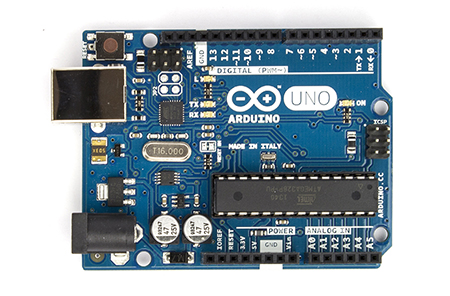
\includegraphics[scale=1.2]{assets/arduino}  
	\end{figure}
\end{frame}

\begin{frame}
	\frametitle{Space}
	\begin{figure}
		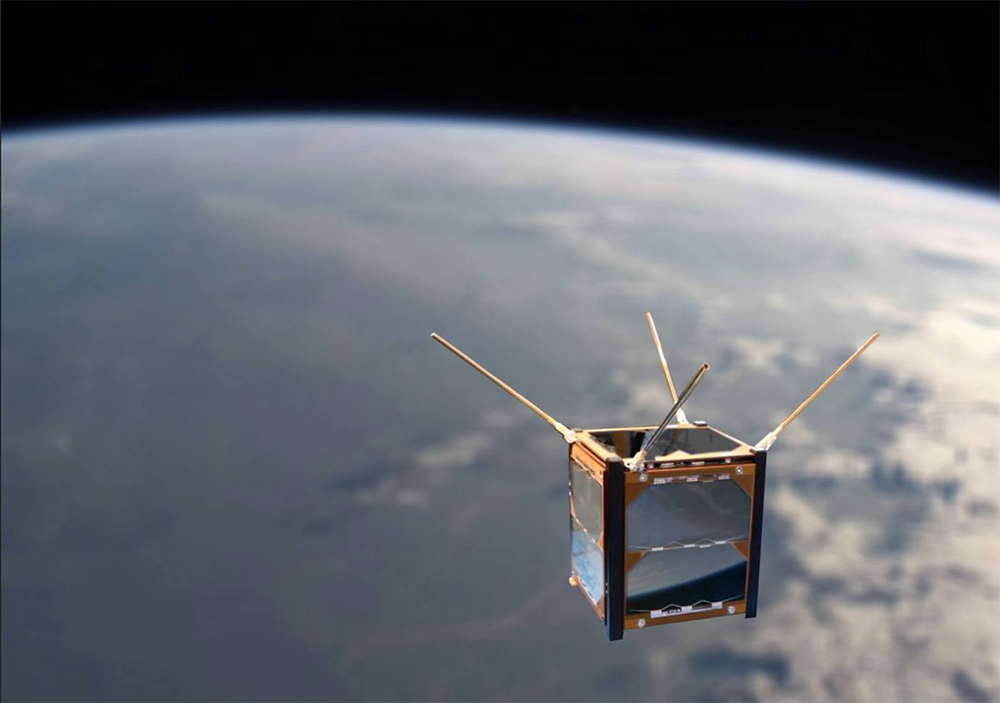
\includegraphics[scale=.4]{assets/sat}  
	\end{figure}
	The ArduSat satellites are powered by the Arduino Uno. It follows cube satellite (CubeSat) standards to build compact 10 cm cubes that can easily be sent to orbit. 
\end{frame}

\begin{frame}
	\frametitle{Sea}
	\begin{figure}
		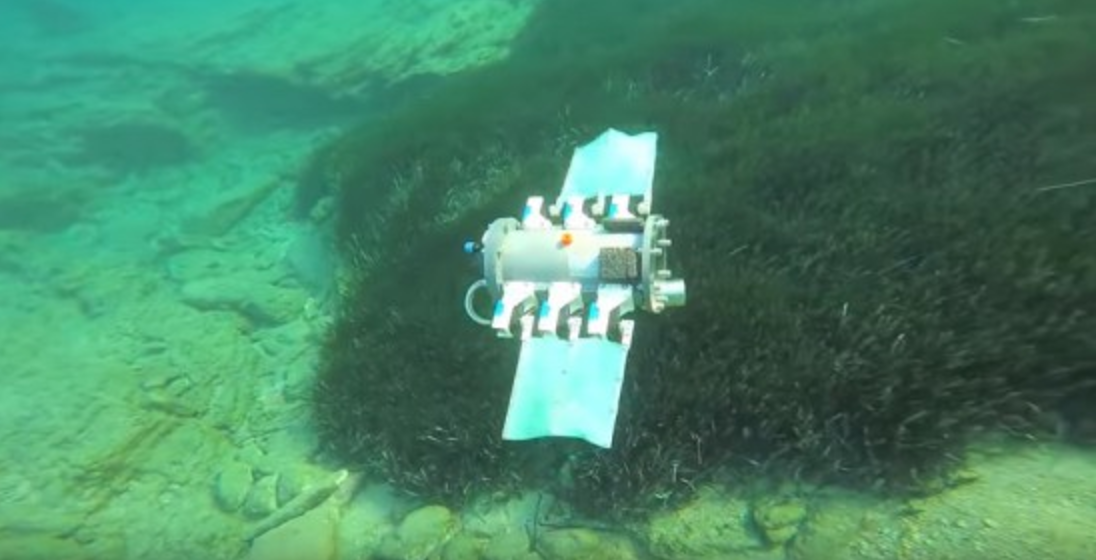
\includegraphics[scale=.4]{assets/sea}  
	\end{figure}
	The robotic prototype swimming under water propelled by fins, it was developed at the Control Systems and Robotics Laboratory of the Technological Educational Institute of Crete, in Heraklion (Greece) and it?s controlled by an Arduino Mega.
\end{frame}


\begin{frame}
	\frametitle{Sensors \& Actuators}
	\begin{figure}
		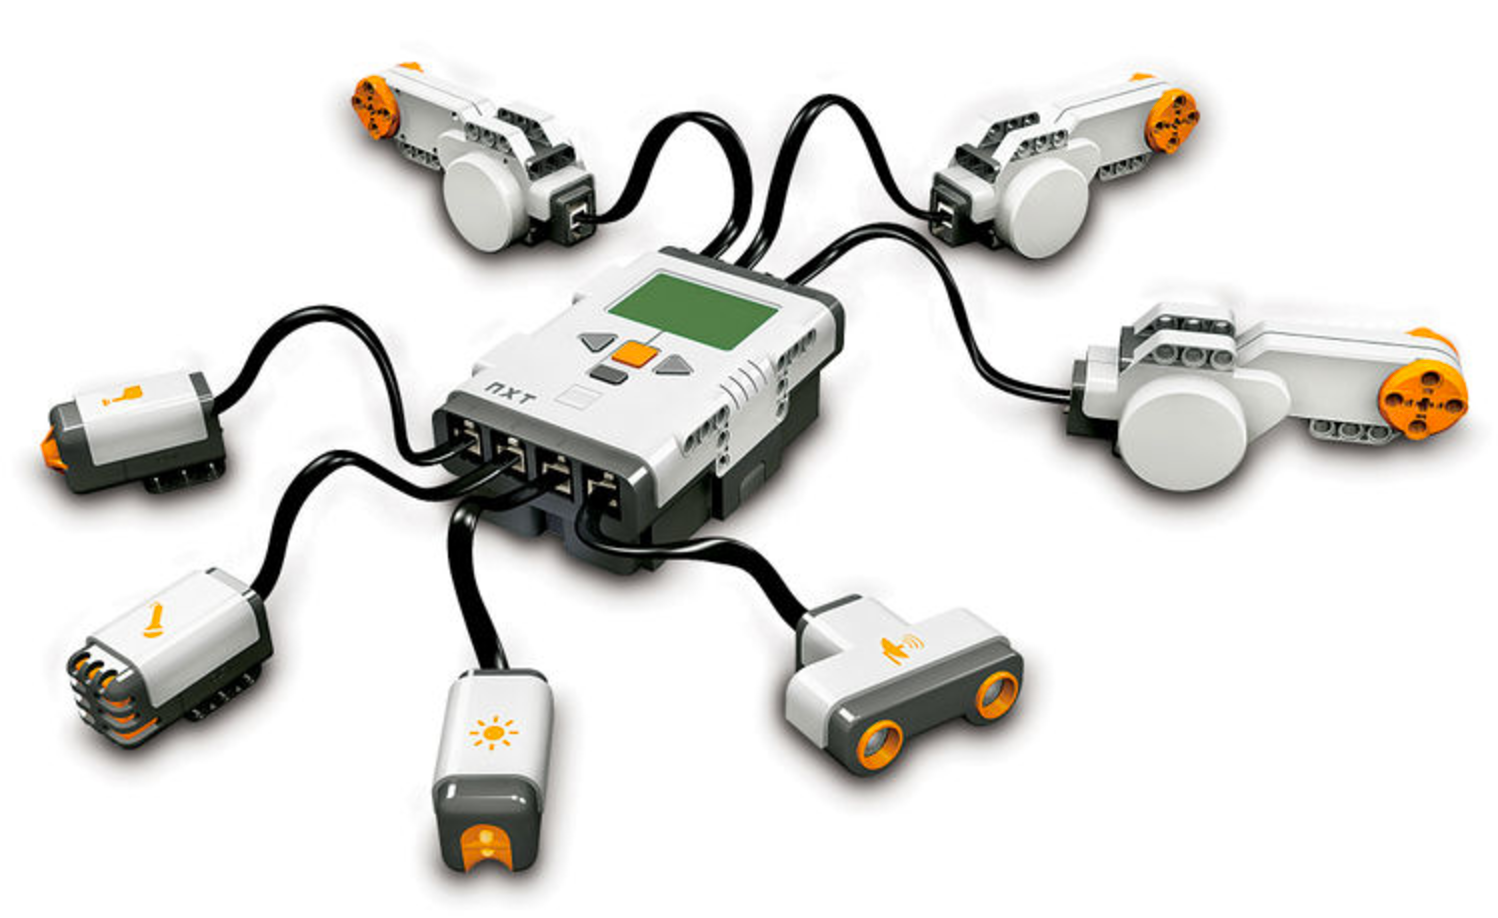
\includegraphics[scale=.15]{assets/nxt}  
		\caption{Just another input / output controller }
	\end{figure}
\end{frame}


\begin{frame}
  \frametitle{What is an Arduino?}
  \begin{itemize}
    \item Open Source
    \item The Arduino is a small microcontroller board
    \item Basically, a small computer 
    \item Perfect for rapid prototyping physical computing systems
    \item Arduino Uno is based on the Atmel ATmega328P
  \end{itemize}
\end{frame}



\begin{frame}
  \frametitle{The basics}  
  The Arduino can only prcesses electronic signals. This means that stimuli from the physical world need to be transduced to electrical signals before they can be processed from within your code. 
  
  \begin{itemize}
    \item 14 Digital IO pins (0-14)
    \item 6 Analogue in pins(0-5)
    \item 6 Analogue out pins(3,5,6,9,10, and 11) ~
  \end{itemize}
\end{frame}

\begin{frame}
	\frametitle{Technical specs}
	\begin{figure}
		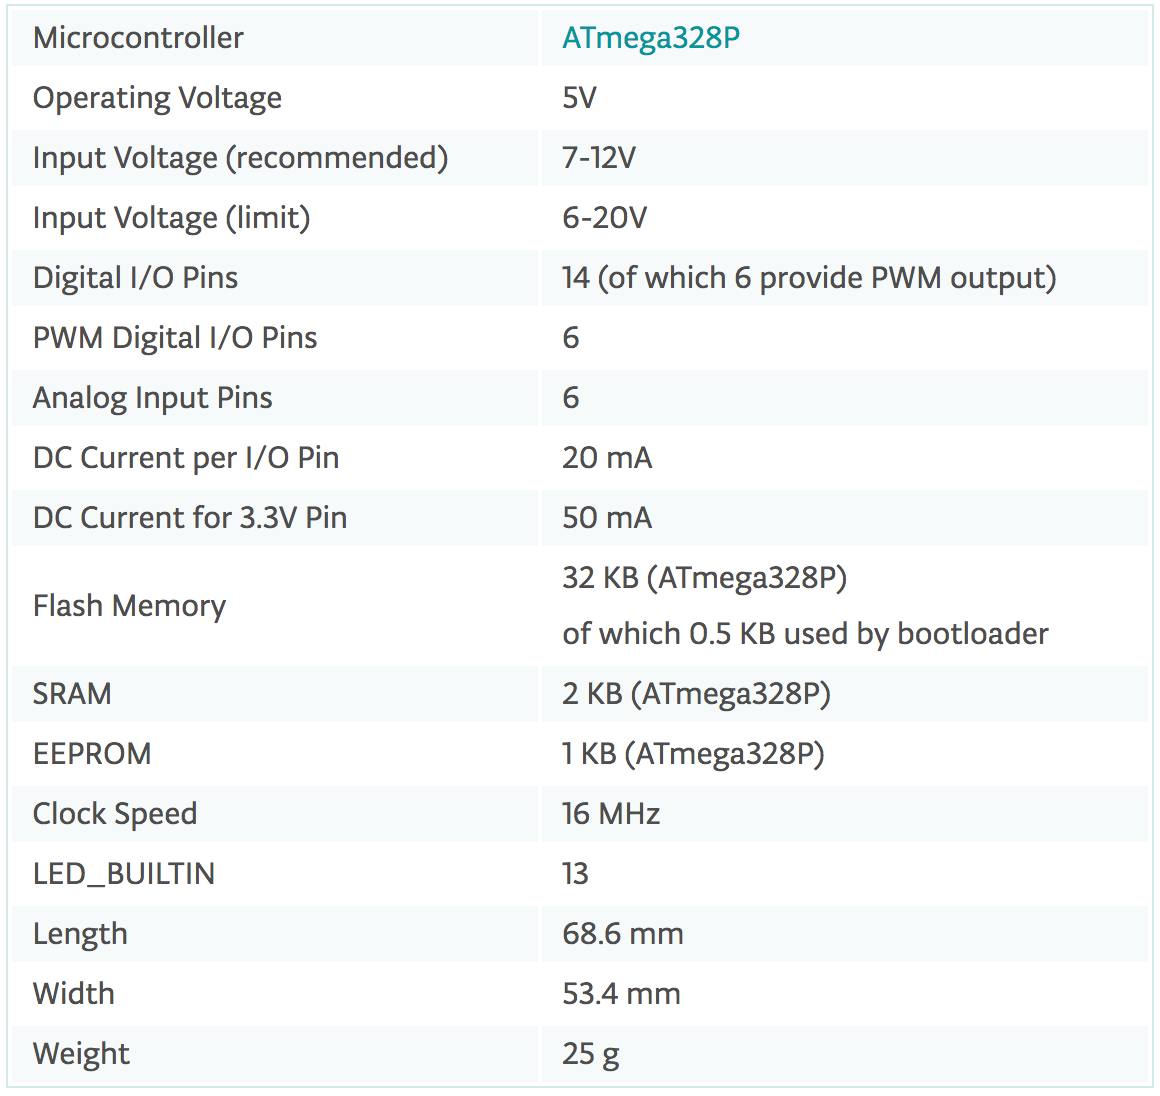
\includegraphics[scale=.14]{assets/spec} 
		\caption{A more in depth version of what the Arduino Uno has to offer}
	\end{figure}
\end{frame}

\begin{frame}
	\frametitle{Memory}
	\begin{itemize}
		\item Flash memory (program space), is where the Arduino sketch is stored.
		\item SRAM (static random access memory) is where the sketch creates and manipulates variables when it runs.
		\item EEPROM is memory space that programmers can use to store long-term information.	
	\end{itemize}
\end{frame}


\begin{frame}
  \frametitle{Power}
	You can power the board using a USB port or DC power supply such as a 9v battery. The Arduino will default to the external power supply if there is one available.   
	\begin{figure}
		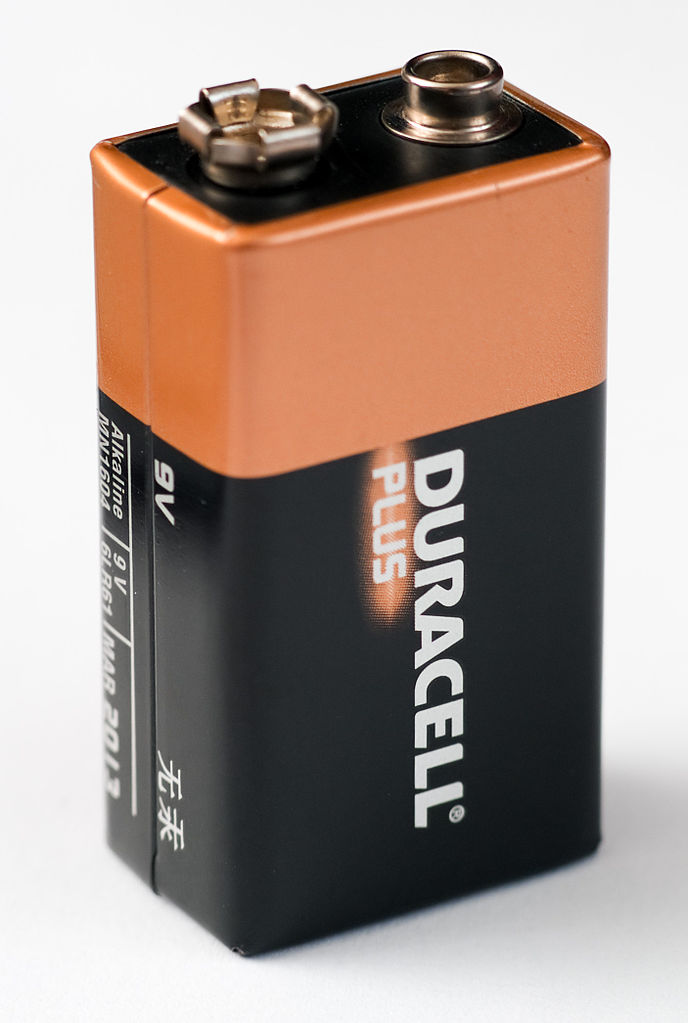
\includegraphics[scale=.1]{assets/battery} 
		\caption{Arduino can be powered by a DC supply 7-12v but all signals are processed at 5v}
	\end{figure}
\end{frame}

\begin{frame}
	\frametitle{Analogue vs. Digital Signal}
	What is the difference? 
	
	\pause
	 \begin{figure}
		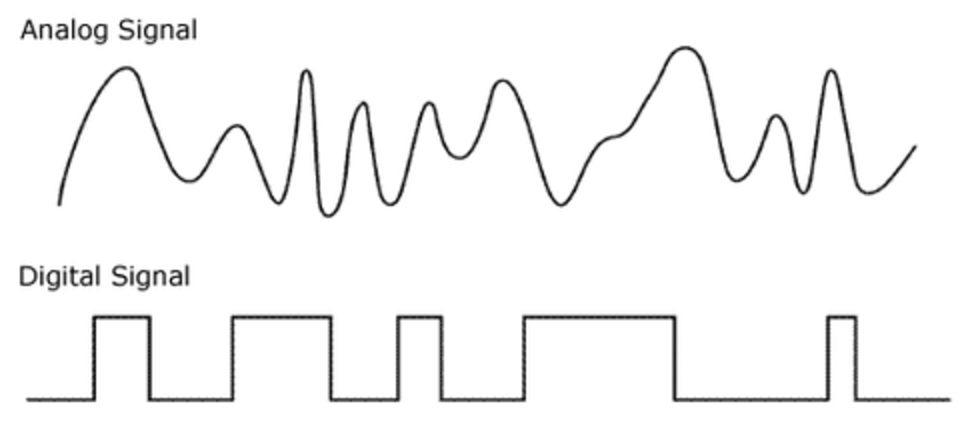
\includegraphics[scale=.25]{assets/dva} 
		\caption{Arduino can be powered by a DC supply 7-12v}

	\end{figure}
\end{frame}

\begin{frame}
	\frametitle{Analogue Out - PWM}
	\begin{figure}
   		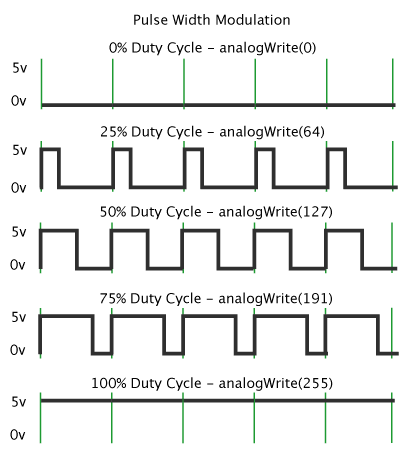
\includegraphics[scale=.4]{assets/pwm} 
	\end{figure}
\end{frame}

\begin{frame}
	\frametitle{Serial Communication}
	Serial communication on pins TX/RX uses TTL logic levels (5V or 3.3V depending on the board). \\~\\
	It communicates on digital pins 0 (RX) and 1 (TX) as well as with the computer via USB. Thus, if you use these functions, you cannot also use \\~\\pins 0 and 1 for digital input or output. 
	Serial is used for communication between the Arduino board and a computer or other devices. 
	
\end{frame}

\begin{frame}
	\frametitle{Arduino}
	
	 \begin{figure}
		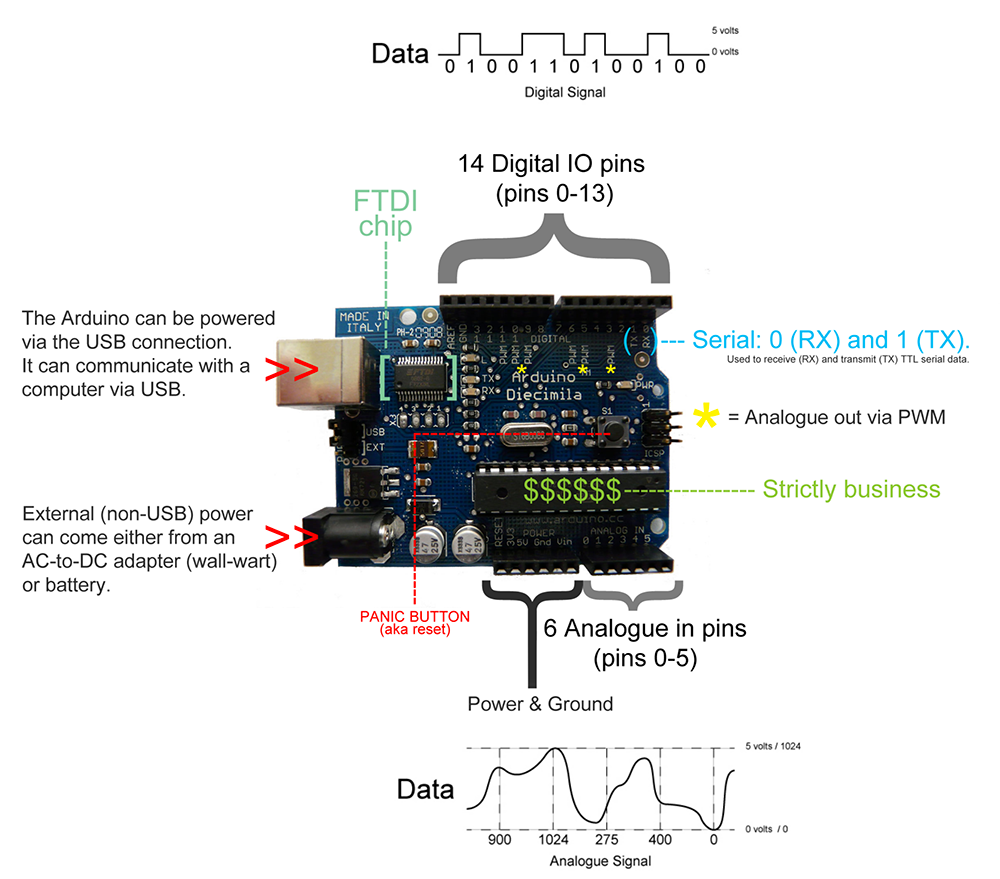
\includegraphics[scale=.2]{assets/map} 
	\end{figure}
\end{frame}

\begin{frame}
	\frametitle{DIY Arduino}
	
	 \begin{figure}
		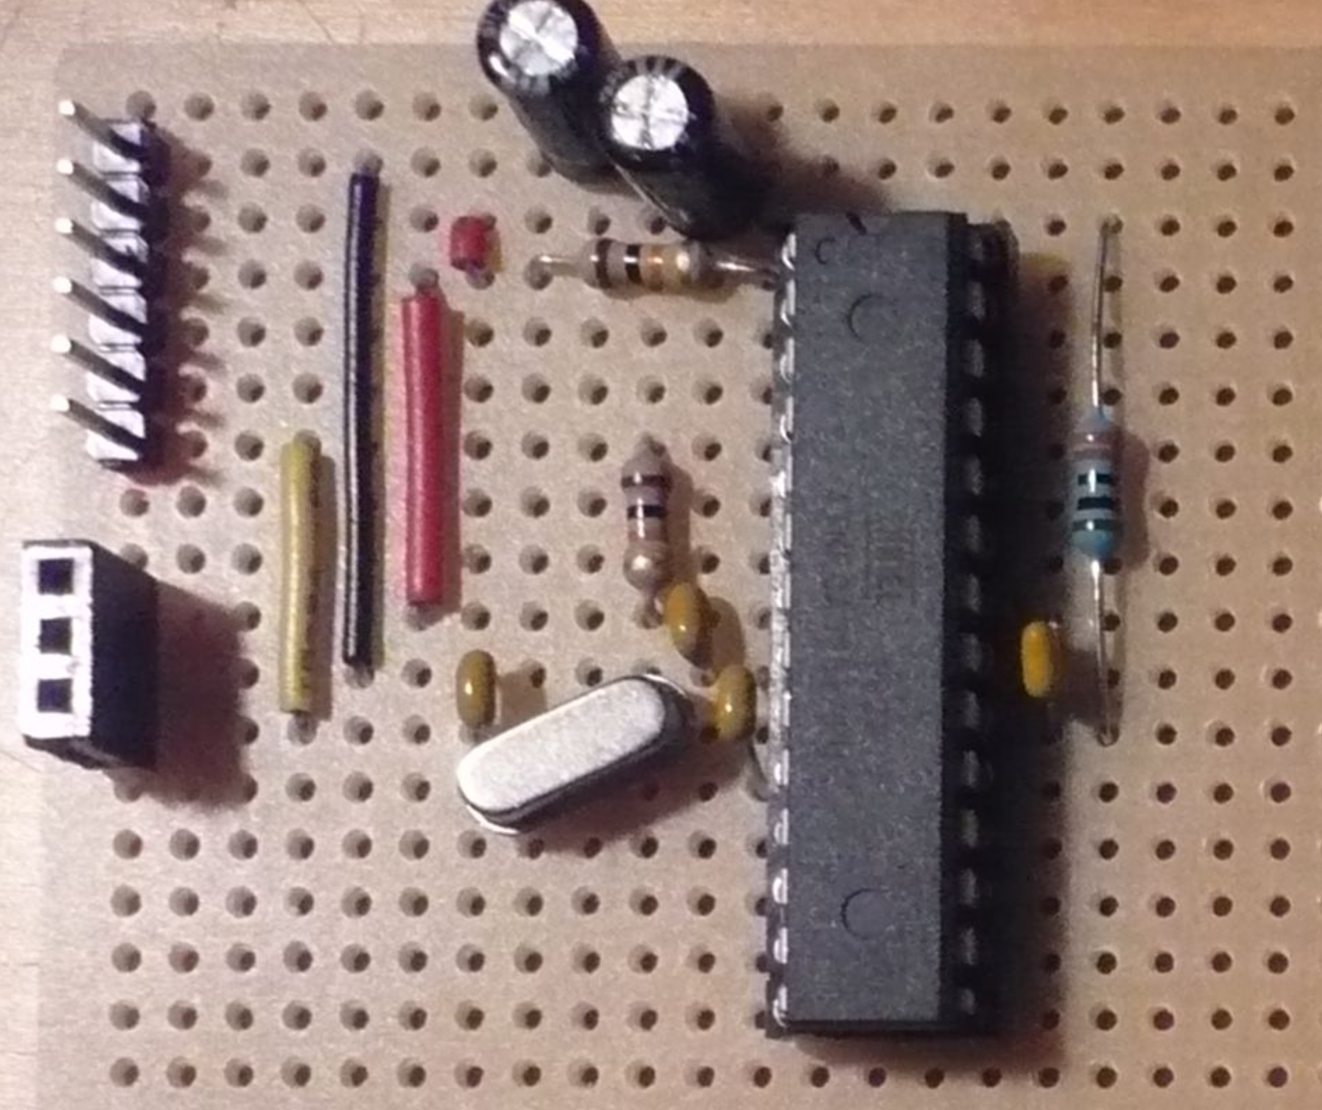
\includegraphics[scale=.2]{assets/diy} 
	\end{figure}
\end{frame}

%SHIELDS 

\begin{frame}
	\frametitle{Shields}
	\begin{figure}
		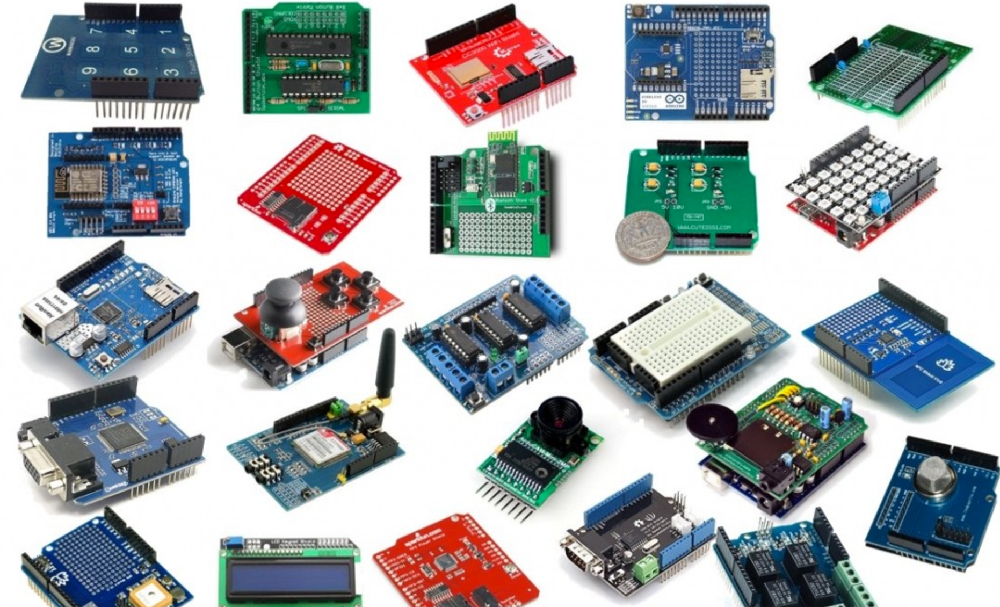
\includegraphics[scale=.28]{assets/shields} 
	\end{figure}
\end{frame}

\begin{frame}
	\frametitle{Open Source Game Boy Clone}
	\begin{figure}
		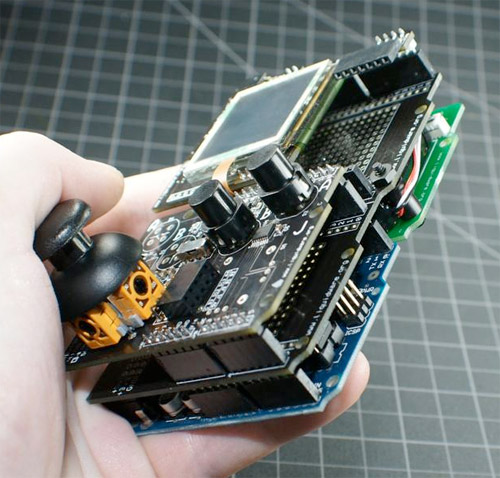
\includegraphics[scale=.32]{assets/gameboy} 
	\end{figure}
\end{frame}

% SENSORS 

%COMPONENTS



\begin{frame}
	\frametitle{Shops}
	\frametitle{Places to buy components}
	\begin{figure}
		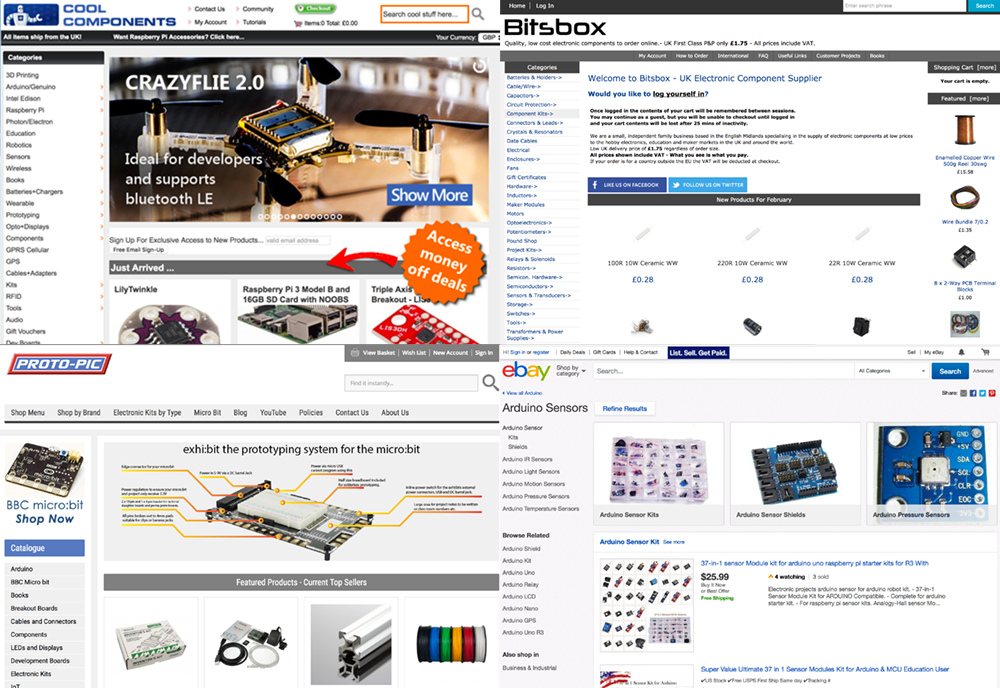
\includegraphics[scale=.25]{assets/shops} 
		\caption{Insure that you buy your components from UK sellers, especially on Ebay}
	\end{figure}
\end{frame}

\begin{frame}
 	\frametitle{Ohms Law - Comic}
   	\begin{figure}
   		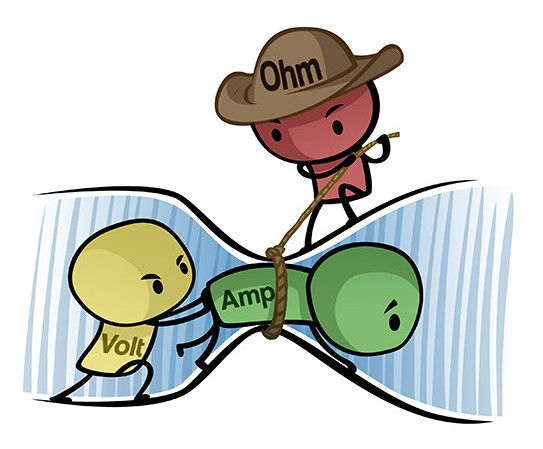
\includegraphics[scale=.3]{assets/ohm} 
	\end{figure}
\end{frame}

\begin{frame}
	\frametitle{Driving Large Loads}
	See spec
	\begin{figure}
   		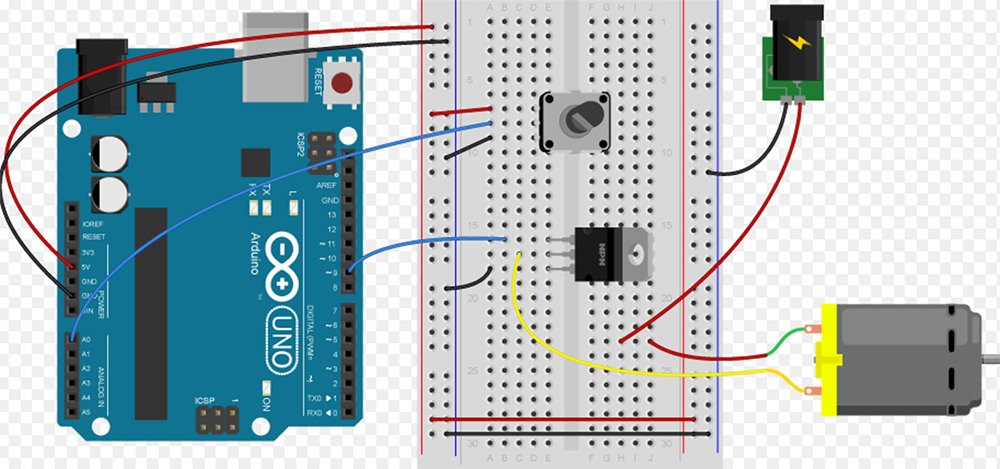
\includegraphics[scale=.6]{assets/loads} 
	\end{figure}
\end{frame}

\begin{frame}
	\frametitle{Reverse Voltage}
	The Arduino should be protected from reverse voltage of solenoids, relays, motors and any other component that use coils. This can be done using a Diode. They act as a one way valve to channel the electric back into the coils. 
	\begin{figure}
   		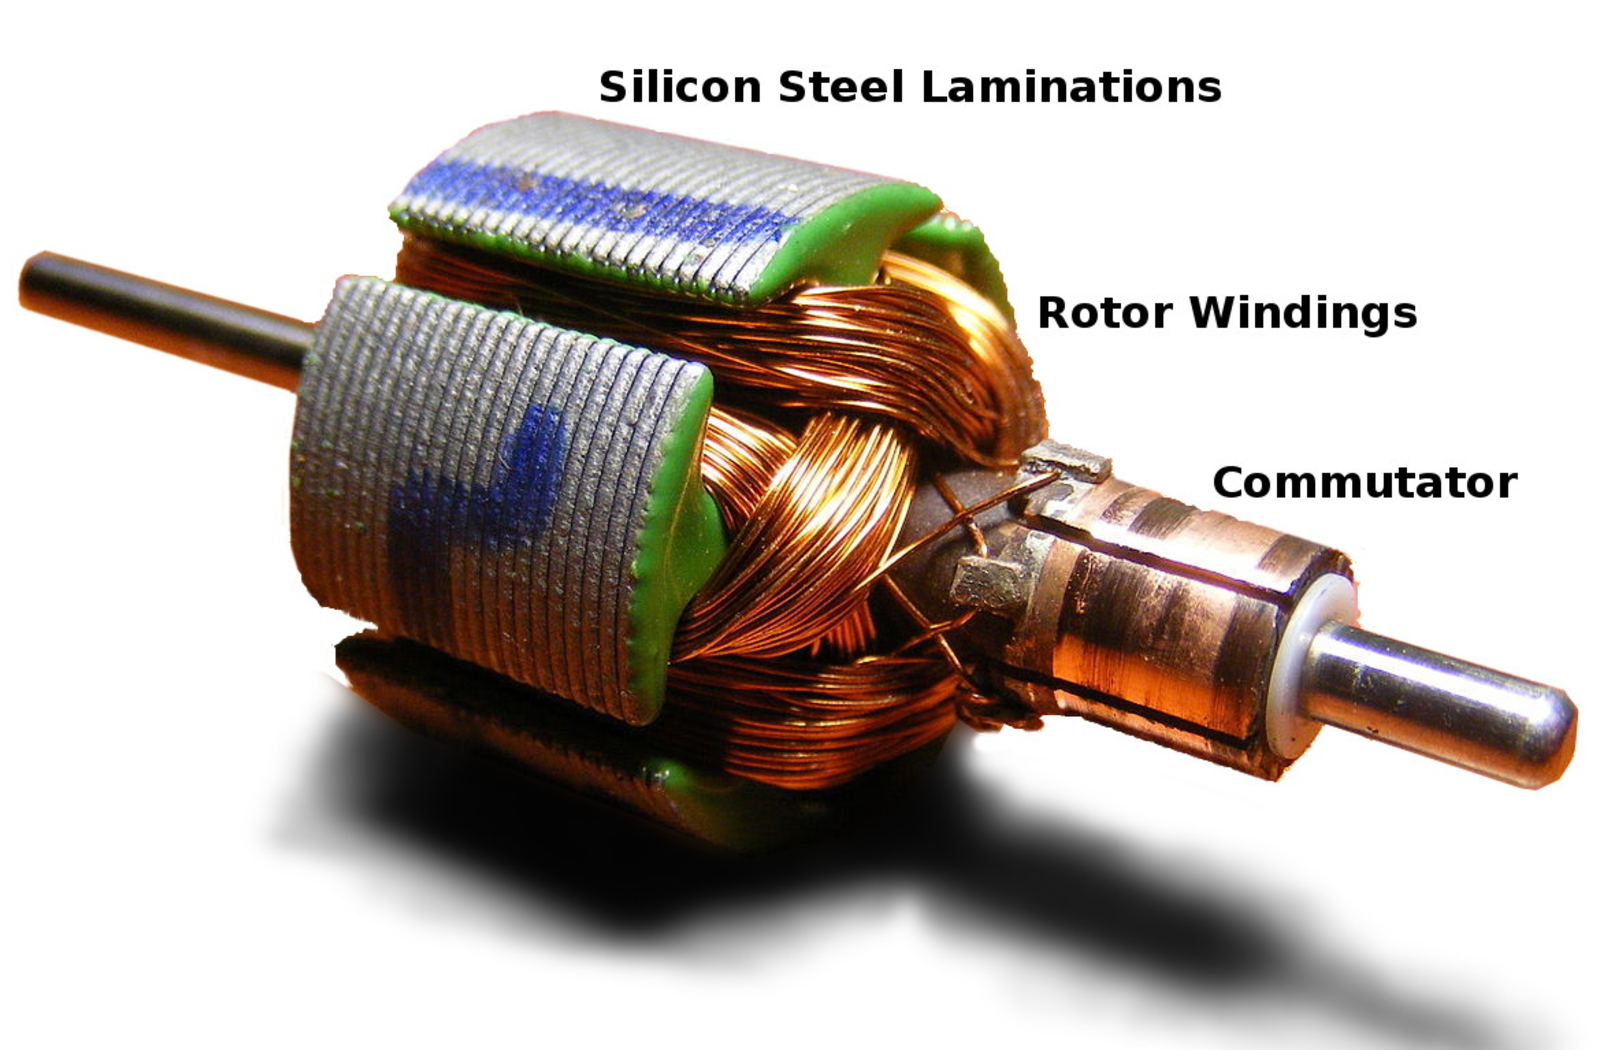
\includegraphics[scale=.2]{assets/motor} 
	\end{figure}
\end{frame}

\begin{frame}
 	\frametitle{Mains Electricity}
   	\begin{figure}
   		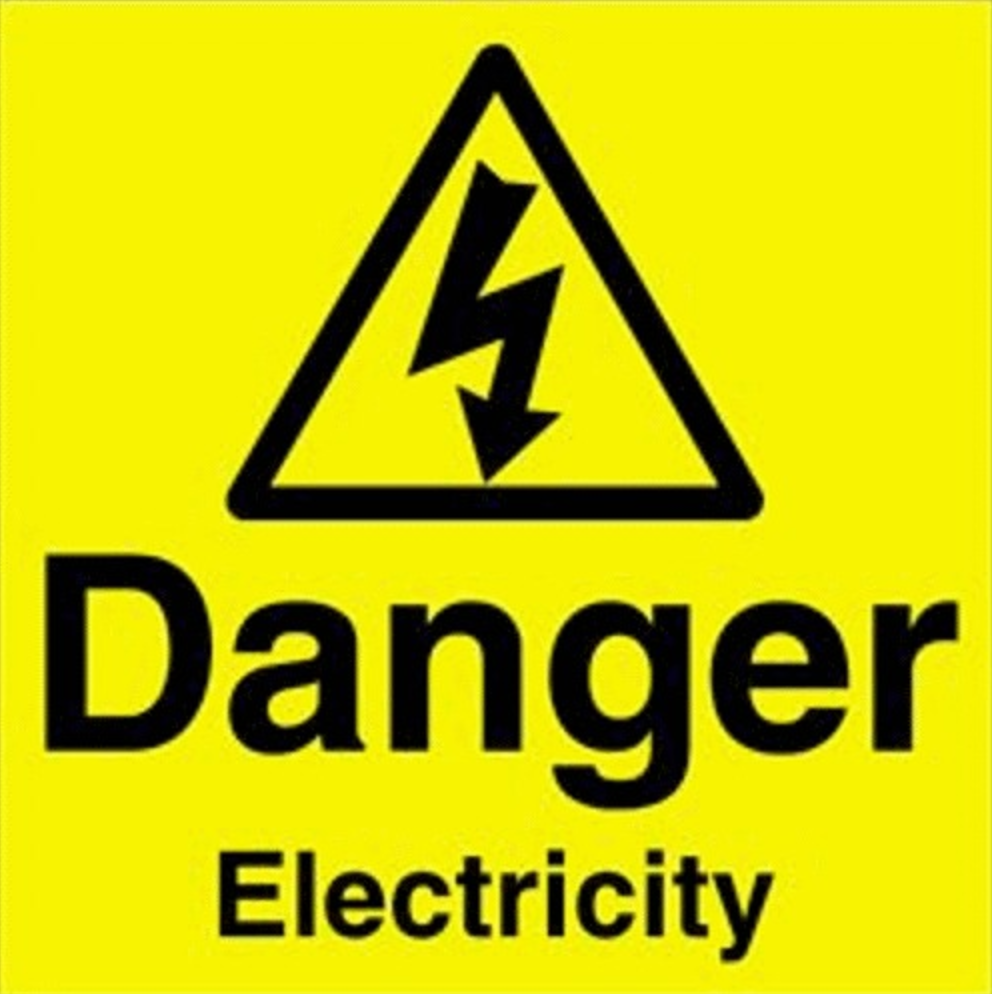
\includegraphics[scale=.3]{assets/240} 
		\caption{There is never any reason why you should be working with mains electricity supply - stay below 12v and even then take care.}
	\end{figure}
\end{frame}

\begin{frame}
 	\frametitle{Programming for Arduino}
	The Arduino language is merely a set of C/C++ functions that can be called from your code. Your sketch undergoes minor changes (e.g. automatic 	generation of function prototypes) and then is passed directly to a C/C++ compiler (avr-g++). \\~\\   
	\url{https://www.arduino.cc/en/Reference/HomePage}
	
\end{frame}

\begin{frame}
	\frametitle{HELLO ARDUINO}
	\begin{figure}
   		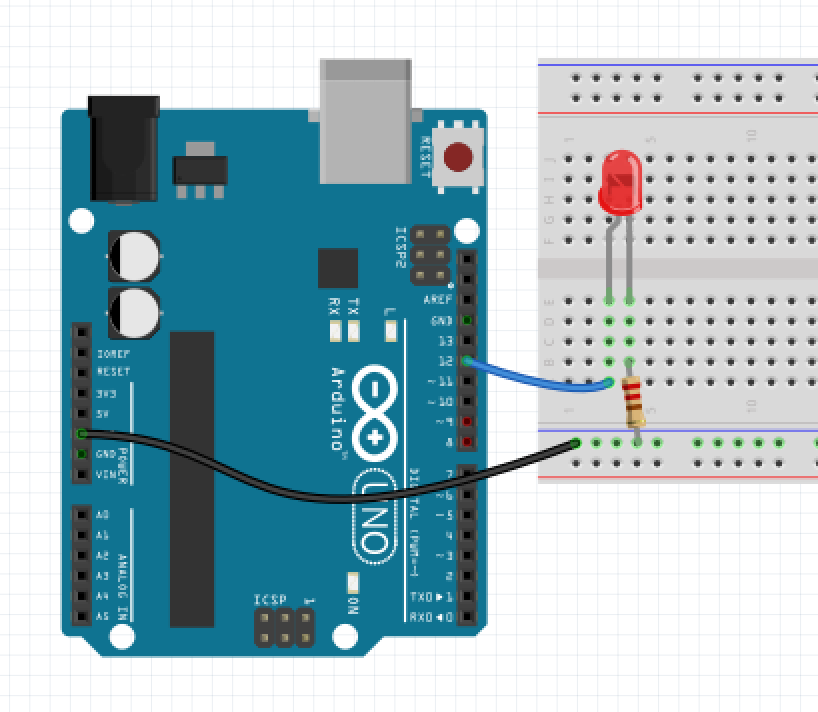
\includegraphics[scale=.55]{assets/hello} 
	\end{figure}
\end{frame}

\begin{frame}
	\frametitle{Resistor}
	\begin{figure}
   		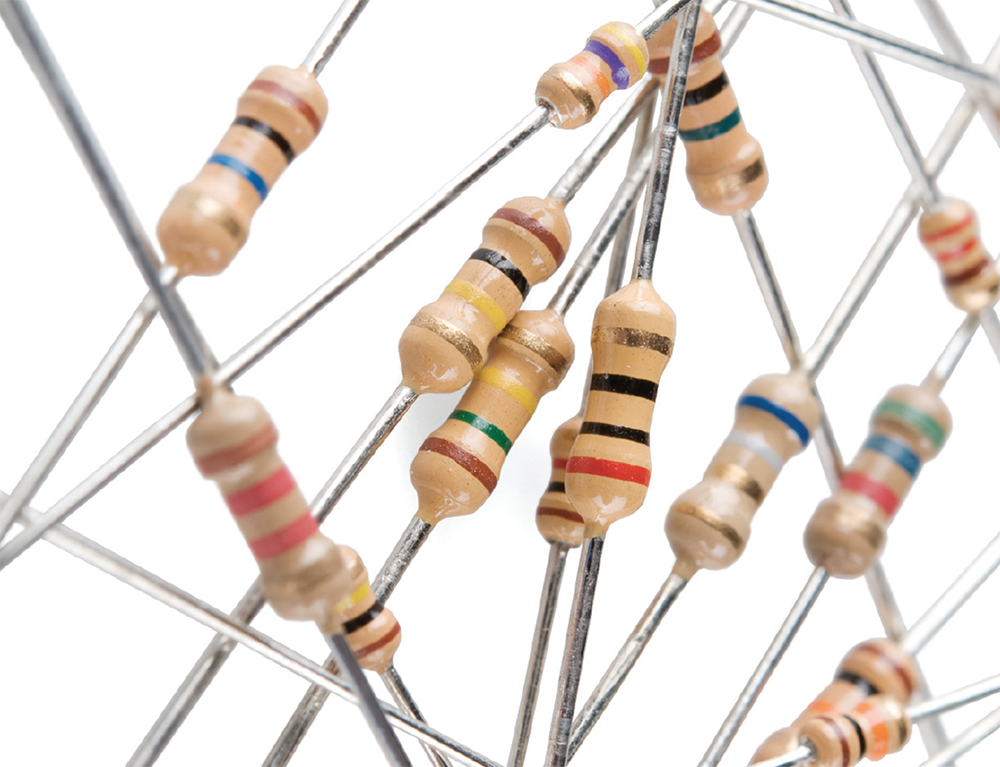
\includegraphics[scale=.2]{assets/resistor} 
	\end{figure}
	In electronic circuits, resistors are used to reduce current flow, adjust signal levels and divide voltages.
\end{frame}

\begin{frame}
	\frametitle{LED}
	\begin{figure}
   		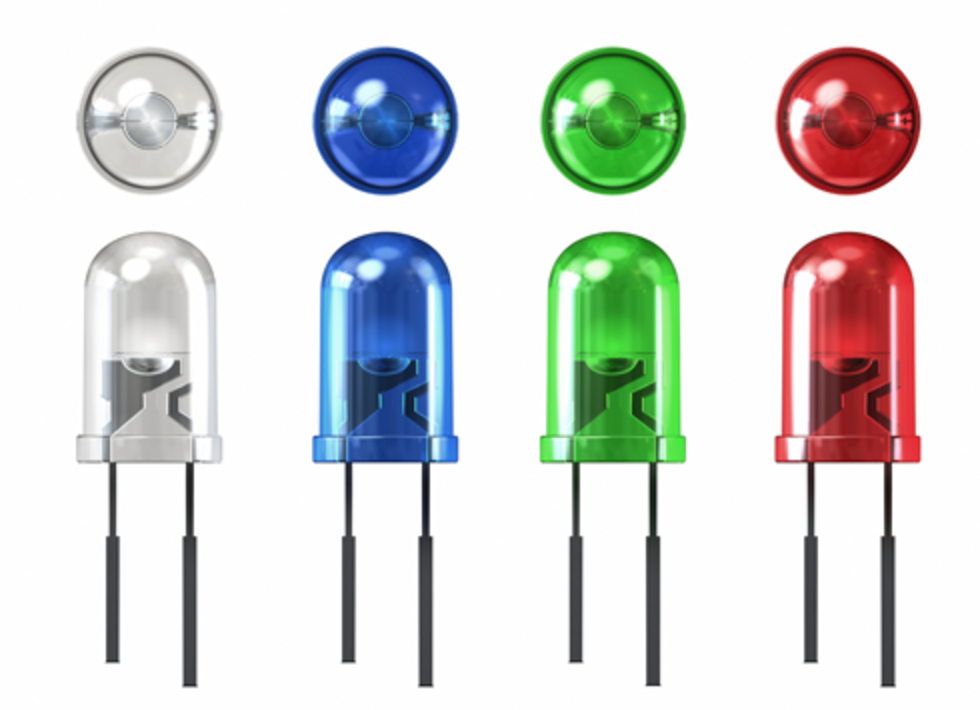
\includegraphics[scale=.2]{assets/led} 
	\end{figure}
	LEDs, being diodes, will only allow current to flow in one direction. And when there's no current-flow, there's no light. Luckily, this also means that you can't break an LED by plugging it in backwards. Rather, it just won?t work.
\end{frame}

\begin{frame}
	\frametitle{Potentiometer}
	\begin{figure}
   		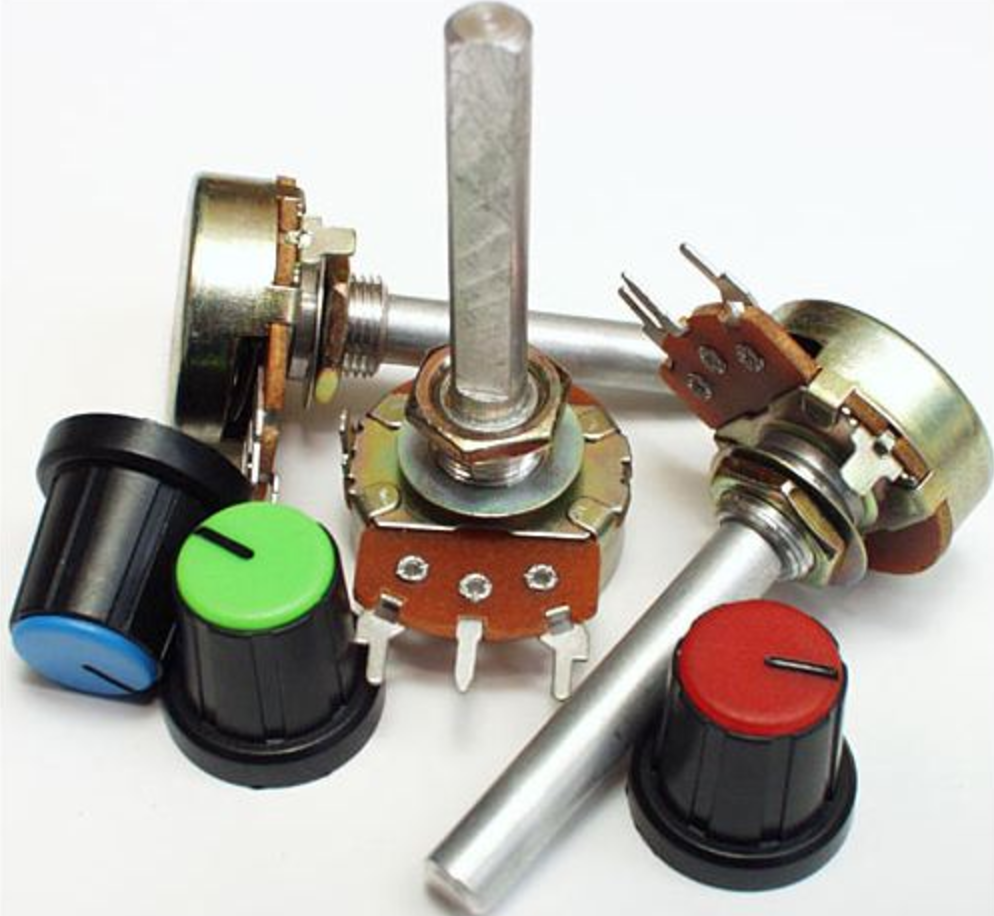
\includegraphics[scale=.2]{assets/pot} 
	\end{figure}
		Potentiometer is a small sized electronic component whose resistance can be adjusted manually. Increasing or decreasing the value of resistance controls the amount of current flowing in a circuit.
	
	
\end{frame}

\begin{frame}
	\frametitle{Button}
	\begin{figure}
   		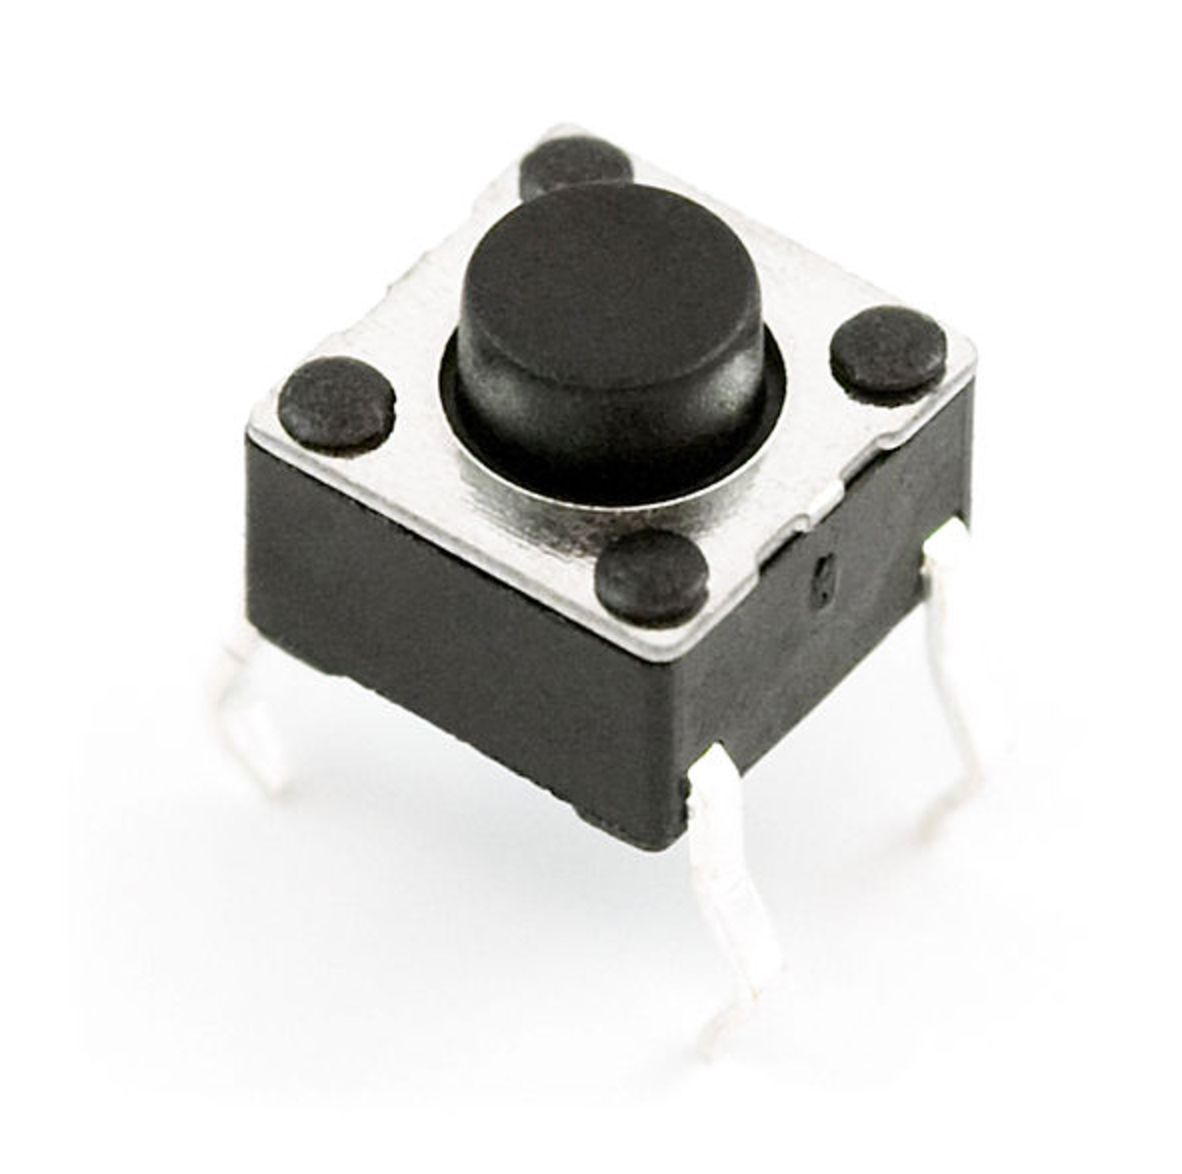
\includegraphics[scale=.2]{assets/butt} 
	\end{figure}
	A device for making and breaking the connection in an electric circuit.
\end{frame}



\end{document}
